\documentclass[12pt, paper=a4]{article}
\usepackage[utf8]{inputenc}
\usepackage[german]{babel}
\usepackage{amsmath}
\usepackage{amssymb}
\usepackage{listings}
\usepackage{graphicx}
\usepackage{fancyhdr}

\author{Mareike Göttsch, 6695217, Gruppe 2\\Paul Hölzen, 6673477, Gruppe 1\\Sven Schmidt, 6217064, Gruppe 1}

\title{AD Hausaufgaben 3}

\rhead{M. Göttsch, G-2; P. Hölzen, G-1; S. Schmidt, G-1}
\pagestyle{fancy}
\begin{document}
\maketitle

\section*{Aufgabe 1.3}
\subsection*{1.}
$L(A_{2.3}) = (ab)^* + cd^*$\\
$L^\omega(A_{2.3}) = (ab)^\omega \cup cd^\omega$\\

\subsection*{2.}
$L^\omega(A_{2.3})$ ist die zweite in Teilaufgabe 1 beschriebene Sprache. Ein beispielhaftes Wort ist: $w_1 = (ab...ab)^\omega$. Die Sprache $(L(A_{2.3}))^\omega$ hingegen akzeptiert Wörter der Form $((ab)^* + cd^*)^\omega$, wie zum Beispiel $w_2 = (ab...ab)\cdot c \cdot d^\omega$. Der Unterschied besteht darin das die erstgenannte Sprache nur entweder eine unendliche Folge von $ab$ oder ein $c$ gefolgt von undendlich vielen $d$s enthält, während die zweite Sprache auch beliebige Kombinationen der beiden Teile in einem unendlich ĺangen Wort beinhaltet.\\

\subsection*{3.}
Der Automat der die Sprache $(L(A_{2.3}))^\omega$ akzeptiert ist in Abbildung 1 zu sehen.\\

\begin{figure}[h!]
\centering
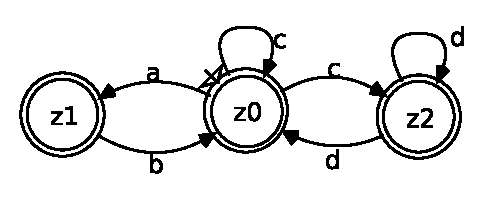
\includegraphics[scale=0.7]{Aufgabe1-4-3.pdf}
\caption{Automat $A_1$}
\end{figure}

\newpage
Um zu zeigen, dass die akzeptierte Sprache dieses Automaten die selbe ist, wie die aus Teilaufgabe 2 müssen wir zwei Richtungen zeigen.\\

1. $L(A_1) \subseteq (L(A_{2.3}))^\omega$\\
Der Automat $A_1$ ist ein Büschi-Automat und akzeptiert so Wörter die ihn mindestens einen der Endzustände unendlich oft durchlaufen lassen. Dies ist der Fall wenn entweder eine Folge von $ab...ab$, eine Folge von $c...c$ oder ein $c$ gefolgt von beliebig vielen oder keinen $d$s gelesen wird. Dies entspricht genau der $\omega$-regulären Menge $L^\omega(A_{2.3}) = (ab)^\omega \cup cd^\omega$.\\

2. $(L(A_{2.3}))^\omega \subseteq L(A_1)$\\
In der Menge $(L(A_{2.3}))^\omega$ sind drei Arten von Wörtern enthalten. Erstens unendliche Folgen von $ab...ab$. Diese werden vom Automaten $A_1$ akzeptiert, da der Endzustand $z1$ uunendlich oft durchlaufen wird. Zweitens Wörter die mit einem $c$ beginnen und von beliebig vielen oder keinen $d$s gefolgt sein können. Auch diese werden vom Automaten akzeptiert, da bei Wörtern, die unendlich viele $c$s enthalten, der Endzustand z0 unendlich oft durchlaufen wird, werden ein oder mehrere $d$s dahinter gelesen, durchläuft der Automat $z2$ unendlich oft. Drittens sind in der Sprache $(L(A_{2.3}))^\omega$ auch Wörter enthalten, die unendlich lang sind und beliebige Kombinationen der ersten beiden Varianten enthalten. Da in den zuvor genannten beiden Varianten immer mindestens ein Endzustand durchlaufen wird, besucht eine unendliche Folge dieser Wortteile mindestens einen Endzustand unendlich oft.\\

Damit gilt $(L(A_{2.3}))^\omega = L(A_1)$.

\section*{Aufgabe 1.4}
Dass die gemischte Konkatenation $W \cdot U \subseteq \Sigma^\omega$ ist, lässt sich durch die Konstruktion eines Büschi-Automaten zeigen, der die Konkatenation zweier Sprachen $W$ und $U$ akzeptiert wobei $W$ eine reguläre Sprache ist und $U$ eine $\omega$-reguläre Sprache.\\
\\
Gegeben diese Sprachen $W$ und $U$ lässt sich ein DFA konstruieren, der $W$ akzeptiert und ein Büschi-Automat, dessen akzeptierte Sprache $U$ ist. Diese Automaten können zusammengefügt werden, indem jede Kante $(s_0, s_1)$ im DFA die in einen der Endzustände führt ($s_1 \in F$ des DFA) im Konkatenationsautomaten entfernt wird und dafür Kanten $(s_0, t)$ für alle $t \in Q_0$ des (nichtdeterministischen) Büschi-Automaten hinzugefügt werden. Die Endzustände des DFA werden entfernt und die Startzustände des Büschi-Automaten zu normalen Zuständen.\\
\\
Übergibt man dem so entstandenen Automaten ein Wort $\sigma = w \cdot u$, mit $w \in W$ und $u \in U$, so durchläuft der erste Teil $w$ des Wortes den Teil der aus dem DFA übernommen wurde, bis schließlich das letzte Zeichen, bei dem dieser einen Endzustand erreicht hätte, in einen der Startzustände des Büschi-Automaten führt. Der hintere Teil $u$ des Wortes ist ein unendlich langes $\omega$-reguläres Wort, das nach der Konstruktion des Konkatenationsautomaten mindestens einen der Endzustände unendlich oft durchläuft. Da diesem Teil des Automaten nur Kanten hinzugefügt wurden, die in die Startzustände hineinführen, aber nicht aus dem Büschi-Automaten hinaus, ändert sich das Verhalten nicht und der Automat akzeptiert das Wort.\\
\\
Das hier beschriebene Verfahren Terminiert in endlicher Zeit, da sowohl der DFA als auch der Büschi-Automat, die hier als Eingabe dienen, eine endliche Anzahl an Zuständen und Kanten haben.\\
\\
Da ein Büschi-Automat existiert der Wörter der Form $\sigma = w \cdot u$ akzeptiert, ist somit auch die Sprache $W \cdot U \subseteq \Sigma^\omega$ also $\omega$-regulär.\\
\end{document}